\documentclass[12pt]{extarticle}
%Some packages I commonly use.
\usepackage[portuguese]{babel}
\usepackage{graphicx}
\usepackage{framed}
\usepackage[normalem]{ulem}
\usepackage{amsmath}
\usepackage{amsthm}
\usepackage{amssymb}
\usepackage{amsfonts}
\usepackage{enumerate}
\usepackage[utf8]{inputenc}
\usepackage{float}
\usepackage{gensymb}
\usepackage[top=1 in,bottom=1in, left=1 in, right=1 in]{geometry}
\usepackage{multirow}
\usepackage{caption}
\usepackage{subcaption}
\usepackage[utf8]{inputenc}
\usepackage{hyperref}

%A bunch of definitions that make my life easier
\newcommand{\matlab}{{\sc Matlab} }
\newcommand{\cvec}[1]{{\mathbf #1}}
\newcommand{\rvec}[1]{\vec{\mathbf #1}}
\newcommand{\ihat}{\hat{\textbf{\i}}}
\newcommand{\jhat}{\hat{\textbf{\j}}}
\newcommand{\khat}{\hat{\textbf{k}}}
\newcommand{\minor}{{\rm minor}}
\newcommand{\trace}{{\rm trace}}
\newcommand{\spn}{{\rm Span}}
\newcommand{\rem}{{\rm rem}}
\newcommand{\ran}{{\rm range}}
\newcommand{\range}{{\rm range}}
\newcommand{\mdiv}{{\rm div}}
\newcommand{\proj}{{\rm proj}}
\newcommand{\R}{\mathbb{R}}
\newcommand{\N}{\mathbb{N}}
\newcommand{\Q}{\mathbb{Q}}
\newcommand{\Z}{\mathbb{Z}}
\newcommand{\<}{\langle}
\renewcommand{\>}{\rangle}
\renewcommand{\emptyset}{\varnothing}
\newcommand{\attn}[1]{\textbf{#1}}
\theoremstyle{definition}
\newtheorem{theorem}{Theorem}
\newtheorem{corollary}{Corollary}
\newtheorem*{definition}{Definition}
\newtheorem*{example}{Example}
\newtheorem*{note}{Note}
\newtheorem{exercise}{Exercise}
\newcommand{\bproof}{\bigskip {\bf Proof. }}
\newcommand{\eproof}{\hfill\qedsymbol}
\newcommand{\Disp}{\displaystyle}
\newcommand{\qe}{\hfill\(\bigtriangledown\)}
\setlength{\columnseprule}{1 pt}
\usepackage[utf8]{inputenc}

\title{Introdução à Dinâmica e Leis de Newton}
\author{Felipe Salvador}
\date{Atualizado em \today}

\begin{document}

\maketitle

\section{Introdução}

Nessa aula, começamos a segunda parte do curso, que será a maior número de aulas e possui o maior número de questões, em média, nos vestibulares.  O nome desse assunto que iremos tratar é: \textbf{Dinâmica}.

Na primeira parte do curso, estudamos os movimentos possíveis, as suas características (velocidade, posição, tempo, aceleração). Agora, iremos ver o porquê desses movimentos acontecem, o que induz a esses movimentos acontecerem.

Na Dinâmica, a pedra fundamental são as \textbf{Leis de Newton}, que são um conjunto de 3 conceitos. A partir dessas 3 leis, conseguimos descrever os mais diversos problemas da Mecânica (parte toda responsável por blocos, massas, rodas, inclinações). Mas, antes de sairmos usando as 3 leis, vamos entender como cada lei funciona.

\section{Leis de Newton}

Isaac Newton (1643-1727) é o físico/astrônomo/matemático que fundou a Física Clássica, responsável por estudar o mundo macroscópico (o nosso mundo). As suas 3 leis iniciaram toda uma série de trabalhos sobre como movimento das coisas é feito. Depois dele, os físicos/matemáticos Joseph-Louis Lagrange (1736-1813) e William Rowan Hamilton (1805-1865) complementaram o seu trabalho com teorias com bases matemáticas mais robustas, em que elas conseguiam descrever objetos e movimentos mais complexos e de forma mais geral. Mas, mesmo as teorias de Lagrange e Hamilton, partem das 3 Leis de Newton com início.

As 3 Leis de Newton são as seguintes:

\begin{itemize}
    \item \textbf{Lei da Inércia} - o seu enunciado é o seguinte: \textbf{“Todo corpo continua em seu estado de repouso ou de movimento uniforme em uma linha reta, a menos que seja forçado a mudar aquele estado por forças aplicadas sobre ele.”} 
    
    Essa lei nos diz que, a menos de uma força (puxar, empurrar), as coisas ficam como estão e ela podem estar em 2 maneiras: paradas ou em movimento. Ou seja, o que está em movimento, continua em movimento (nem a velocidade muda) e o que está parado, continua parado. Não é possível parar ou fazer andar um objeto, sem empurrá ou puxá-lo.
    
    Além disso, a Lei da Inércia nos diz que \textbf{quanto maior a massa dos objetos, mais difícil é mudar o seu movimento}, ou seja, é mais fácil empurrar/freiar uma bicicleta do que um carro ou caminhão. Portanto, essa lei nos traz o significado físico de '\textit{massa}', \textbf{que é uma grandeza que nos diz o quão fácil ou difícil é alterar o seu movimento}, seja esse movimento é estar parado ou não.
    
    \item \textbf{Princípio Fundamental da Dinâmica} - essa é a estrela das 3 Leis de Newton, porque ela relaciona as Forças aplicadas num objeto de interesse, com a massa dele e uma quantidade que vimos em cinemática: a aceleração. Essa segunda lei é descrita como:
    
    \textbf{“A mudança de movimento é proporcional à força motora imprimida e é produzida na direção de linha reta na qual aquela força é aplicada.”}
    
    Com "\textit{mudança de movimento}", entendemos como aceleração. O que essa lei nos diz é que: \textbf{Quanto maior a aceleração que um corpo sofre, maior a força aplicada sobre ele e que a aceleração tem a mesma direção e sentido que a força aplicada (ou seja, a aceleração aponta para o mesmo lugar que a força)}.
    
    Existe uma expressão matemática que relaciona tudo isso:
    
    \begin{equation}\label{eq:newton_vec}
        \Vec{F} = m\,\Vec{a}
    \end{equation}
    
    Quando só estamos olhando para o tamanho da força e da aceleração, a segunda Lei de Newton tem a seguinte forma\footnote{Na verdade, a segunda Lei de Newton relaciona a força resultante com a variação de uma quantidade chamada de \textit{Quantidade de Movimento (no ensino médio) ou momento linear (no ensino superior)} dividida pela variação do tempo: $\Vec{F} = \frac{\Delta \Vec{p}}{\Delta t} \quad \Vec{p} = m\Vec{v}$
    
    Como nos nossos exercícios, a massa dos nossos objetos é constante, a fórmula fica como a dada. Mas para problemas de foguete ou de trem sendo carregados/descarregados em movimento, a massa deixa de ser constante e essa formulação em relação a quantidade de movimento é a mais correta.} :
    
    \begin{equation}\label{eq:newton_scalar}
        |\Vec{F}| = m|\Vec{a}| \implies F=ma
    \end{equation}
    
    
    Nessa expressão, $\Vec{F}$ é a força resultante aplicada, $m$ é a massa do objeto que estou olhando, $\Vec{a}$ é aceleração que esse objeto sofre. Uma questão interessante é que dados 2 das 3 informações, nós podemos encontrar a informação que falta.
    
    Uma questão importante nessa formulação é que $\Vec{F}$ é a força resultante, ou seja, é a soma de todas as forças aplicadas no objeto:
    
    \begin{equation}
        \Vec{F} = \Vec{F}_1 + \Vec{F}_2 + \Vec{F}_3 + \dots
    \end{equation}
    
    No Sistema Internacional, a unidade de força é \textbf{Newton(N)} e ela é dada por:
    
    \begin{equation}
        \left[F \right] = [m][a] \implies N = kg\,\frac{m}{s^2}
    \end{equation}
    
    \newpage
    \item  \textbf{Lei de Ação e Reação} - a nossa última lei é dada assim: \textbf{“A toda ação há sempre uma reação oposta e de igual intensidade: as ações mútuas de dois corpos um sobre o outro são sempre iguais e dirigidas em sentidos opostos.”}
    
    Para explicar essa lei, vou usar o exemplo de empurrar a parede: Quando você empurra a parede, você é jogado para trás. O que isso quer dizer é que quando um corpo 1 aplica uma força sobre corpo 2, acontece uma reação que o corpo 2 empurra o corpo 1 com a mesma intensidade para outro lado.
    
    Isso é formulado da seguinte forma:
    
    \begin{equation}
        \Vec{F}_{12} = - \Vec{F}_{21}
    \end{equation}
    
    \noindent em que $\Vec{F}_{12}$ é a força que o corpo 1 faz no corpo 2 e $\Vec{F}_{21}$ é a força de reação que o corpo 2 faz no corpo 1.
    
    Um outro exemplo é como nós andamos e pulamos:
    
    \begin{figure}[H]
        \centering
        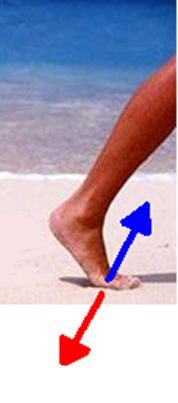
\includegraphics[width=0.15\textwidth]{caminhado-sobre-a-areia.jpg}
        \caption{Diagrama de forças na caminhada. Para irmos para frente, nós fazemos uma força para trás e para baixo, de forma que o chão reaja empurrando a gente para cima e para frente.}
        \label{fig:walk}
    \end{figure}
    
    Sempre que 2 corpos interajam (um empurre o outro), sempre há um par ação e reação. Mas às vezes, um corpo tem muito mais massa que o outro, então o corpo que tem mais massa não se move ou muda, como é o caso de nós empurrarmos uma parede. A parede tem muito mais massa que nós, então quando empurramos ela, ela não se move, mas pela reação, a gente é jogado para trás.
    
\end{itemize}

Vamos a 2 exemplos para ilustrar as Leis de Newton:

\textbf{Exemplo 1:} Um corpo, inicialmente em repouso, de 2 kg de massa e sofre uma força de 4N. Qual é a aceleração que esse corpo sofre?

\begin{align*}
    &F = ma\\
    &4 = 2*a \implies a = 2 m/s^2
\end{align*}
\textit{Extra: usando as equações da cinemática, encontre a velocidade final desse objeto, sabendo que ele percorreu 100m. Gabarito: V=20m/s}

\textbf{Exemplo 2:} Um corpo de 10 kg em movimento começa a sofrer uma frenagem, cuja aceleração é de $2 m/s^2$. Qual é a força que essa frenagem está aplicando?

Como é uma frenagem, então a aceleração é negativa.
\begin{align*}
    &F = m*a \\
    &F = 10*(-2) \implies F = -20 N
\end{align*}

\textit{Extra: Se o corpo está inicialmente a uma velocidade de 10 m/s, use as equações da cinemática para encontrar o instante em que o corpo para. Gabarito: t =5s}
\section{Força Peso $\Vec{P}$}

Tem um tipo de força que faz a gente ficar preso na Terra, sem sair voando pelo espaço todo: a Força Peso. Ela é gerada pela gravidade, que é responsável pela atração das massas. A gravidade é um tipo de força que faz as massas se aproximarem e ficarem juntas. É assim que as estrelas, planetas, galaxias são formadas. Veremos no final dessa parte do curso como essa força da gravidade é contabilizada.

A força peso é dada pela seguinte fórmula:

\begin{equation}
    \Vec{P} = m\,\Vec{g}
\end{equation}
\noindent em que $\Vec{g}$ é a aceleração da gravidade (que aponta para o centro da Terra), que na superfície da Terra, ao nível do mar, é aproximadamente:
\begin{equation}
    |\Vec{g}| = g \approx 9,8\, m/s^2
\end{equation}

Essa força é uma especial, porque a aceleração dessa força é constante e tem um valor definido, independentemente do objeto em que a força esteja agindo. Ou seja, se eu soltar uma pena de ave e uma bigorna do topo de um prédio, a princípio, os dois objetos teriam a mesma aceleração e chegariam ao chão no mesmo instante. Mas não é bem isso que vemos na realidade, porque ignoramos a ação de sustentação do ar, que faz com que a pena flutue, enquanto a bigorna caia normalmente.

Mas se eu fizer o mesmo experimento num duto sem ar (vácuo), vejo que ambos chegama ao chão ao mesmo tempo. Isso foi o que Galileu Galillei descobriu lá no século 16. A BBC (canal britânico de tv), fez \href{https://www.youtube.com/watch?v=qSeW0f51QzY}{um documentário (com legendas em portguês - clique aqui)} sobre o  experimento que ele fez para mostrar que os dois objetos chegam ao chão juntos.

\textbf{Exemplo 1:} Calcule a força peso de um objeto de 10 kg.

\begin{align*}
    &P = mg \\
    &P = 10*9,8 \implies P=98 N
\end{align*}


\textit{Extra:} Sabemos que na Terra, a gravidade é o que nos mantém preso a ela. Mas se só existisse a gravidade e a Força peso, nós iríamos ser acelerados até o núcleo da Terra, o que não acontece. 

Então, pela Segunda Lei de Newton, se nós ficamos tranquilos sobre o chão, sem entrar no chão, então a aceleração que sofremos é 0. Portanto, há alguma outra força que cancela a força peso e que faz com que nós não sejamos levados ao centro da Terra. 

Qual é a intensidade dessa força que não nos deixa ser levados até o núcleo, supondo que a nossa massa seja de 70 kg?

\textit{Gabarito: próximas aulas!!!}

\end{document}
